\documentclass[tikz,border=12pt]{standalone}
\usepackage[T1]{fontenc}
\usepackage{mathpazo}
\usepackage{amsmath,amssymb}
\usetikzlibrary{arrows.meta, positioning, calc, decorations.pathreplacing, patterns}

\definecolor{stblue}{HTML}{7B97AD}
\definecolor{rwgold}{HTML}{B8995E}
\definecolor{sage}{HTML}{7A9A7E}
\definecolor{dkbrown}{HTML}{3D3530}
\definecolor{wmgray}{HTML}{7B7067}
\definecolor{cream}{HTML}{F9F6F0}
\definecolor{border}{HTML}{D4C9B8}
\definecolor{terracotta}{HTML}{C47A6A}
\definecolor{lavender}{HTML}{907EA0}

\begin{document}
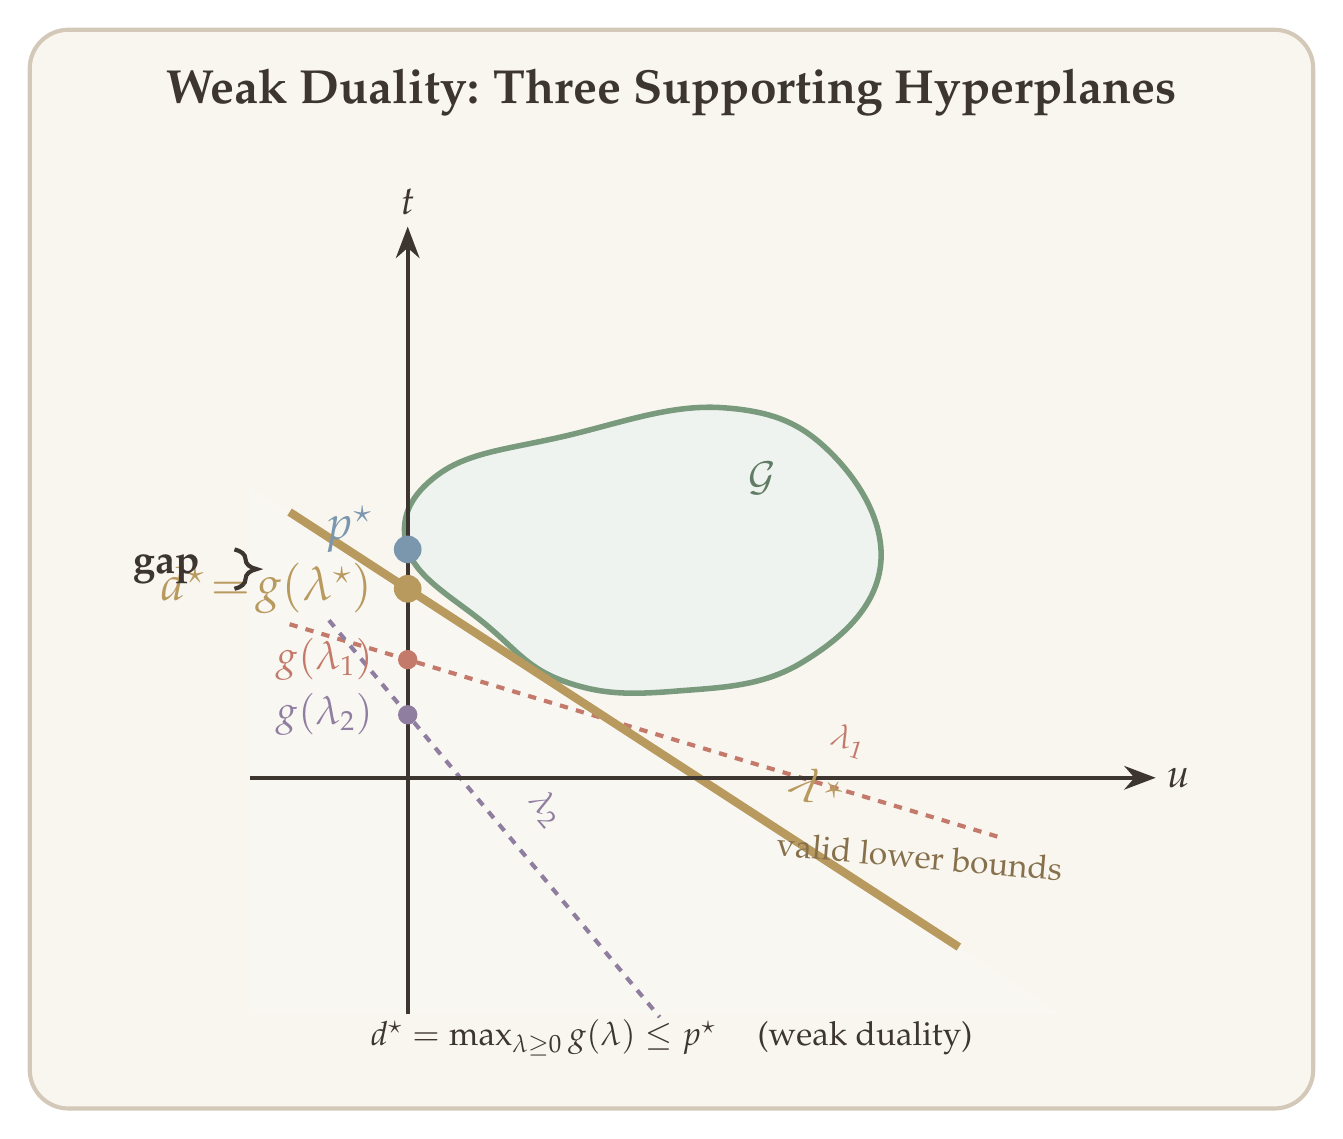
\begin{tikzpicture}[>={Stealth[length=4mm, width=3mm]}, line width=1.5pt]

% Background
\fill[cream, rounded corners=14pt] (-4.8,-4.2) rectangle (11.5,9.5);
\draw[border, line width=1.5pt, rounded corners=14pt] (-4.8,-4.2) rectangle (11.5,9.5);

% Title
\node[font=\LARGE\bfseries, text=dkbrown, align=center] at (3.35,8.7)
  {Weak Duality: Three Supporting Hyperplanes};

% --- Fills and shapes (drawn BEFORE axes) ---

% Light shading below optimal hyperplane
\begin{scope}
\clip (-2,-3) rectangle (9.5,7);
\fill[rwgold!8]
  (-2, {2.4+0.65*2}) -- (9.5, {2.4-0.65*9.5}) -- (9.5,-3) -- (-2,-3) -- cycle;
\end{scope}

% The set G
\fill[sage!12, draw=sage, line width=2pt]
  plot[smooth cycle, tension=0.7] coordinates {
    (0,2.9) (1,1.94) (2,1.22) (3.4,1.1)
    (5,1.46) (6,2.66) (5.4,4.1)
    (4,4.7) (2,4.34) (0.4,3.86)
  };
\node[font=\Large\bfseries, text=sage!80!black] at (4.5,3.8) {$\mathcal{G}$};

% Three hyperplanes (clipped to stay within canvas)
\begin{scope}
\clip (-2.5,-3.5) rectangle (10,7.5);

% lambda_1 (shallow slope, terracotta): slope -0.3, intercept 1.5
\draw[terracotta, line width=1.5pt, dashed]
  (-1.5, {1.5+0.3*1.5}) -- (7.5, {1.5-0.3*7.5});

% lambda* (optimal, rwgold): slope -0.65, intercept 2.4
\draw[rwgold, line width=3pt]
  (-1.5, {2.4+0.65*1.5}) -- (7, {2.4-0.65*7});

% lambda_2 (steep slope, lavender): slope -1.2, intercept 0.8
\draw[lavender, line width=1.5pt, dashed]
  (-1, {0.8+1.2*1}) -- (3.2, {0.8-1.2*3.2});

\end{scope}

% --- Axes (drawn AFTER fills so they remain visible) ---
\draw[->, dkbrown, line width=1.5pt] (-2,0) -- (9.5,0)
  node[right, font=\Large, text=dkbrown] {$u$};
\draw[->, dkbrown, line width=1.5pt] (0,-3) -- (0,7)
  node[above, font=\Large, text=dkbrown] {$t$};

% --- Line labels (along visible portions) ---
\node[font=\large, text=terracotta, rotate=-17, anchor=south]
  at (5.5, {1.5-0.3*5.5+0.3}) {$\lambda_1$};
\node[font=\LARGE\bfseries, text=rwgold, rotate=-33, anchor=south]
  at (5, {2.4-0.65*5+0.4}) {$\lambda^\star$};
\node[font=\large, text=lavender, rotate=-50, anchor=south]
  at (1.5, {0.8-1.2*1.5+0.4}) {$\lambda_2$};

% "valid lower bounds" label in shaded region
\node[font=\large, text=rwgold!60!dkbrown, rotate=-5] at (6.5,-1.0)
  {valid lower bounds};

% --- Intercept points and labels on t-axis ---
% g(lambda_2) = 0.8
\fill[lavender] (0,0.8) circle (3.5pt);
\node[font=\Large, text=lavender, left] at (-0.3,0.8) {$g(\lambda_2)$};

% g(lambda_1) = 1.5
\fill[terracotta] (0,1.5) circle (3.5pt);
\node[font=\Large, text=terracotta, left] at (-0.3,1.5) {$g(\lambda_1)$};

% d* = g(lambda*) = 2.4
\fill[rwgold] (0,2.4) circle (5pt);
\node[font=\LARGE\bfseries, text=rwgold, left] at (-0.3,2.4)
  {$d^\star\!=\!g(\lambda^\star)$};

% p* point
\fill[stblue] (0,2.9) circle (5pt);
\node[font=\LARGE\bfseries, text=stblue, left] at (-0.3,3.15)
  {$p^\star$};

% Brace for duality gap
\draw[decorate, decoration={brace, amplitude=8pt}, dkbrown, line width=1.5pt]
  (-2.2,2.9) -- (-2.2,2.4);
\node[font=\Large\bfseries, text=dkbrown, left] at (-2.5,2.65) {gap};

% Bottom annotation
\node[font=\large, text=dkbrown, align=center] at (3.35,-3.3)
  {$d^\star = \max_{\lambda \ge 0} g(\lambda) \le p^\star$ \quad (weak duality)};

\end{tikzpicture}
\end{document}
